\chapter{Results and Interpretation}

\label{cap7}

\textit{In the research of high mass Higgs boson, processes that have been predicted but not yet seen are searched . Given that no excesses over the SM expectation are seen in the mass spectra, the  upper limits on the cross sections are computed. In this chapter  the 95\% CL exclusion limits
on the production cross-section are evaluated. These exclusion limits are also interpreted in term  of 2HDM. I have performed the limits evaluation for the 
fully-leptonic analysis and I have participated in the limit combination among fully- and same-leptonic analysis. }

\section{Statistical interpretation}
\label{StatIn}
The Bayesian and the classical frequentist~\cite{cowan1998statistical}, with a number of modifications, are two statistical approaches commonly used in high energy physics for characterising the absence
of a signal.
Both methods allow one to quantify the level of incompatibility of data with a signal
hypothesis,  which  is  expressed  as  a  confidence  level  (C.L.)~\cite{CMS-NOTE-2011-005}. For excluding a signal the C.L. 95\% is a common choice.
The C.L. probabilistic interpretation is used when stating the non-existence
of a signal is not straightforward and the subject of a vast body of literature as in the high mass analysis.
The procedure used the establish the upper limits calculation is based on frequentist test using  a likelohood ratio as a test statistic. In addition to the parameter of interest such as the cross section of the signal, the signal and the background models contain a nuisances parameters whose values are not take in account as know \textit{a priori} but rather must be fitted from the data ~\cite{Cowan:2010js}.
In the following the frequentist approach is described.  The expected high mass signal  event yields will be generically denoted as $s$ and the backgrounds as $b$.
\newline
The  frequentist approach is built  to discriminate signal from background events. The most powerful statistic test, in according to the Neyman-Pearson lemma~\cite{cowan1998statistical}, is the likelihoods ratio $\lambda (\mu)$, 
\begin{equation}
  \lambda (\mu)=\frac{\mathcal{L}(data | \mu s +b)  }{ \mathcal{L}(data | b) }  \end{equation}
where, $\mathcal{L}$ is the likelihood function from the product of Poisson probabilities and  $\mu$ is the strength of the signal process (the case $\mu =0$ correspond to background only hypothesis, $\mu=1$ the the nominal signal hypothesis).
One can see that $0 \leq  \lambda (\mu) \leq 1 $, $\mu$ near 1 is a evidence of good agreement among data and the hypothesized $\mu$ value.\\
It is convenient, for numerical reason, to use the test statistic $q_{\mu}$ defined as,  
\begin{equation}
 q_{\mu}= -2 \ln \lambda (\mu)  \end{equation}
where high value of $q_{\mu}$ correspond to  more likely incompatibility between data and $\mu$, i.e. background only hypothesis. \\
Using the statistic test  $q_{\mu}$, is possible to quantify the level of disagreement between the data and the hypothesis, $p$-value, defined as,
\begin{equation}
  p_{\mu}=  \int_{ q_{\mu},obs }^{\infty } f(q_{\mu}| \mu  ) dq_{\mu}   \end{equation}
where $ q_{\mu,obs} $ is the value of statistic test $q_{\mu}$ observed from the data and $f(q_{\mu}| \mu  )$ is the pdf of $q_{\mu}$ under the assumption of the signal strength $\mu$.
\newline
The systematic uncertainties on signal $s(\theta)$ and background $b(\theta)$ rates are introduced in test statistic.
The test statistic then would take the following form:
\begin{equation}
 q_{\mu} =\frac{\mathcal{L}(data | \mu, \hat{\theta}_{\mu} )  }{ \mathcal{L}(data |0, \hat{\theta}_0 )},  \end{equation}
where $\hat{\theta}_{\mu}$ and $\hat{\theta}_0$ are maximum likelihood estimators for the signal+background
hypothesis (with the signal strength factor $\mu$) and for the
background-only hypothesis ($\mu =0$). 
The profile likelihood test statistic is introduced to prevent negative signal as,
\begin{equation}
 \tilde{q}_{\mu} =\frac{\mathcal{L}(data | \mu, \hat{\theta}_{\mu} )  }{ \mathcal{L}(data |\hat{\mu}, \hat{\theta} )}, \; \; 0 \leq \hat{\mu} \leq \mu \; ,  \end{equation}
where $\hat{\mu}$ and $\hat{\theta}$ gives the global maximum of the likelihood. 
The constrain  $0 \leq \hat{\mu}$ is due to a positive signal rate, while the   $\hat{\mu} \leq \mu$ is imposed by hand in order to guarantee a one-sided  confidence interval.\\
At this point is useful to evaluate the observed statistic test $\tilde{q}_{\mu}^{obs}$ and the nuisance parameters $\hat{\theta}_0^{obs}$, $\hat{\theta}_{\mu}^{obs}$ that escribing  the  experimentally observed data for the background-only and signal+background hypotheses, respectively.
With this in mind, the pdf of the test statistic in constructed by generating toy MC pseudo-data for both the background-only and signal+background hypotheses, 
$f(\tilde{q}_{\mu}| \mu, \hat{\theta}_{\mu}^{obs}  )$ and $f(\tilde{q}_{\mu}| \mu, \hat{\theta}_{0}^{obs}  )$. The corresponding $p$-value for the
signal+background and background-only hypotheses, $p_{\mu}$ and $p_b$ are given by:


\begin{equation}
  p_{\mu}= P( \tilde{q}_{\mu} \geq \tilde{q}_{\mu}^{obs} | signal+background)=  \int_{ q_{\mu},obs }^{\infty } f(\tilde{q}_{\mu}| \mu, \hat{\theta}_{\mu}^{obs}   ) d \tilde{q}_{\mu}   \end{equation}


\begin{equation}
 1- p_{b}= P( \tilde{q}_{\mu} \geq \tilde{q}_{\mu}^{obs} | background-only)=  \int_{ q_{0},obs }^{\infty } f(\tilde{q}_{\mu}| 0, \hat{\theta}_{0}^{obs}   ) d \tilde{q}_{\mu}.   \end{equation}
The CL$_{s}(\mu)$ is given by the ratio,
\begin{equation}
  CL_s(\mu)=\frac{p_{\mu}}{1-p_b}   \end{equation}
To quote the 95\% of confidence level upper limits on $\mu$, $\mu$ is adjust until reaches CL$_S$=0.05.
For the background-only hypothesis, the expected median upper-limit and $\pm 1 \sigma$ and $\pm 2 \sigma$ bands are generated with a large set   of background-only pseudo-data. The CL$_S$ is evaluated for each of them.
Then,  one can build a cumulative probability distribution of results by starting integration from the side corresponding to low event yield.
The point at which the cumulative probability distribution crosses the quantile of 50\% is the median expected value. 
The  $\pm 1 \sigma$ (68\%) band is defined by the crossings of the 16\% and 84\% quantiles.  Crossings at 2.5\% and 97.5\% define the  $\pm 2 \sigma$ (95\%) band.
\newline
In the high mass analysis,  the interference contribution is not negligible, as described in \ref{sec:interference}, and it is included as part of the signal. 
In particular during the fit the interference term is scaled by $\sqrt{\mu}$.
However, to prevent possible negative probability distribution function of the interference,  during the fit the signal yield is computated as,
\begin{equation}
Yield=\sqrt{\mu} \times (S+B+I)+ (\mu -\sqrt{\mu}) \times (S) + (1-\sqrt{\mu}) \times (B)
\end{equation}
where  $S$ is the signal, $B$ the background and $I$ the interference.


\section{Signal interpretation: EW singlet, 2HDM and MSSM}
\label{sec:signalModel}
The signal is interpreted in terms of the electroweak singlet model, in 2HDM and finally in  MSSM model. The theory part of the models are described in Sec.~\ref{NSP}. 

\subsection*{Electroweak singlet model}
The EW singlet represents a scalar mixing among the high mass particle and the Higgs boson. This model relies on two parameters: the scale factor of the couplings of the high mass resonance with respect to the SM, $C'$, and the branching fraction of the electroweak singlet to non-SM decays modes, $BR_\mathrm{new}$. The electroweak singlet signal strength, $\mu'$ and the modified width, $\Gamma'$, are related with the parameters in the model by the following equations:
\begin{equation}
\mu' = C'^2 \cdot (1 - BR_\mathrm{new})
\end{equation}
\begin{equation}
\Gamma' = \Gamma_\mathrm{SM} \cdot \frac{C'^2}{1 - BR_\mathrm{new}}
\end{equation}
The high mass signal samples for different mass hypothesis have been reweighted according to this model. At the moment only the $BR_\mathrm{new} = 0$ hypothesis has been investigated while we tested different $C'$ values.
In Fig.~\ref{fig:cprime} are shown the \mll and \mt templates corresponding to a high mass boson  of 700\GeV for three different $C'$ values: $C' = 1$, corresponding to the SM Higgs decay width, $C'=0.5$, corresponding to $\Gamma' = 2.5\cdot10^{-2}\,\Gamma_\mathrm{SM}$, and $C'=0.1$, corresponding to $\Gamma' = 10^{-2}\,\Gamma_\mathrm{SM}$. A value of $BR_\mathrm{new} = 0$ is considered in all cases. We note that the signal shape is not very sensitive to different $C'$ values.
\begin{figure}[htbp]
\centering
\subfigure[Simulated LHE signals]{
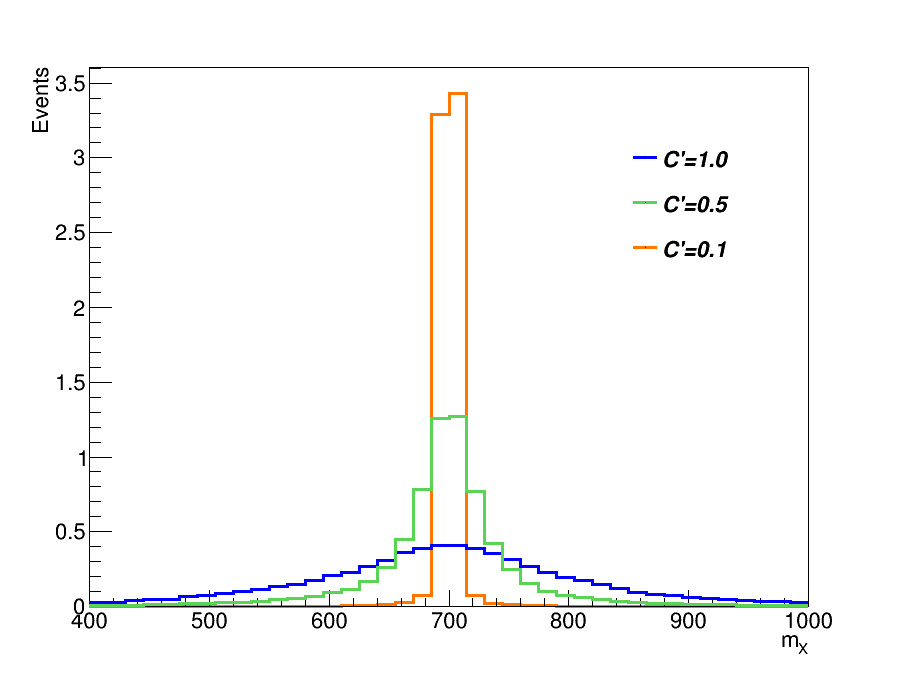
\includegraphics[width=0.45\textwidth]{../AN/Figs/higgsLHEmass700_cuts_nocuts.png}
}
\subfigure[$m_T^H$]{
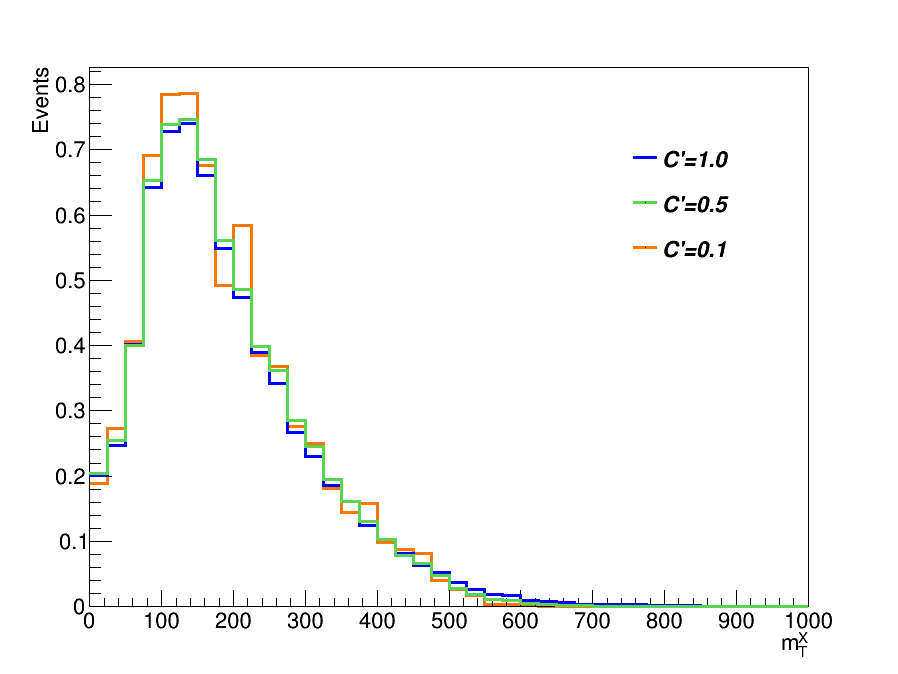
\includegraphics[width=0.45\textwidth]{../AN/Figs/mth700_cuts_nocuts.png}
}
\\
\subfigure[$m_{\ell \ell}$]{
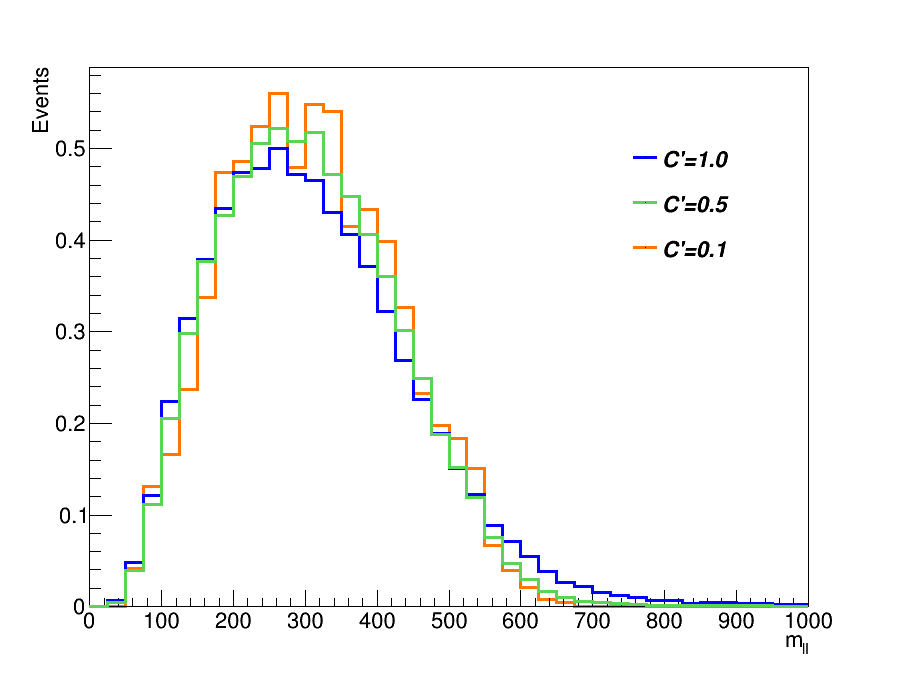
\includegraphics[width=0.45\textwidth]{../AN/Figs/mll700_cuts_nocuts.png}
}
\subfigure[$m_T^I$]{
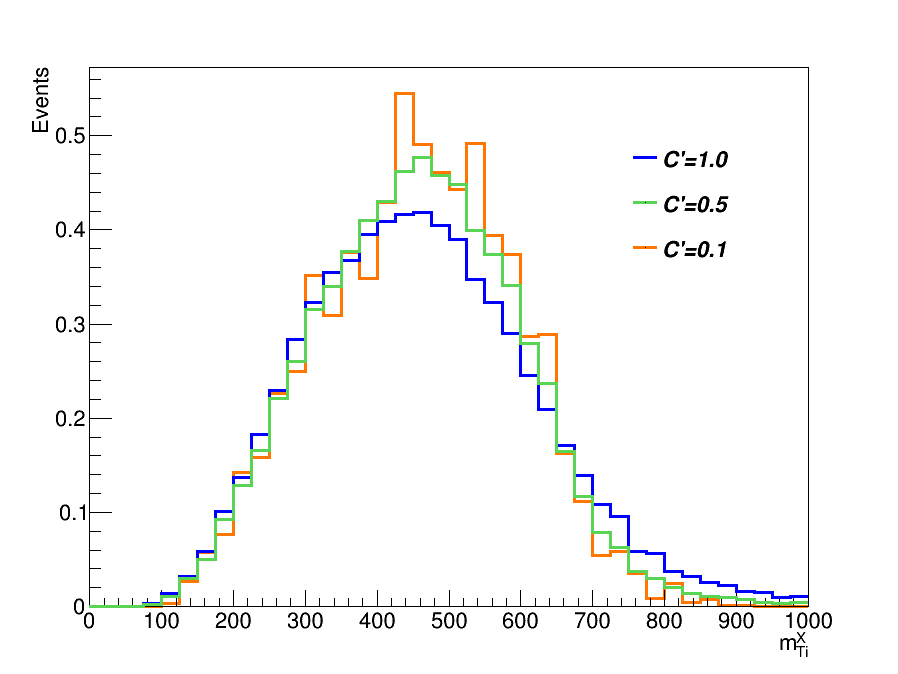
\includegraphics[width=0.45\textwidth]{../AN/Figs/mTi700_cuts_nocuts.png}
}
\caption{ 
    Distributions of the signals, the $m_T^H$, the $m_{\ell \ell}$ and the  $m_T^I$ variables at generator level for different values of $C'$, without any selection.}
    \label{fig:cprime}
\end{figure}

\subsection*{2HDM and MSSM models}
The 2HDM is a well motivated extension of the SM. It contains two Higgs doublets, from which a total of five Higgs bosons are predicted: Two CP-even bosons $h$ and $H$, a CP-odd boson $A$ and two charged bosons $H^\pm$. In most theories, $h$ exhibits the features of the SM Higgs boson, while $H$ is a CP-even Higgs boson at a higher mass. The 2HDM comprises many free parameters. Two of these are of particluar interest:
\begin{itemize}
\item $\tan\beta$: The ratio $\frac{v_u}{v_d}$ of the vacuum expectation values of the two Higgs doublets.
\item $\alpha$: The mixing angle of the two scalar Higgs bosons $h$ and $H$.
\end{itemize}
The quantity $\cos(\beta-\alpha)$ is also of interest, as the coupling of the heavy scalar Higgs boson $H$ to two vector bosons is proportional to this factor. In the decoupling limit, which occurs at $\cos(\beta-\alpha)=0$, all couplings become SM-like.
A 2HDM of type-2 is considered in this study. Here up-type quarks couple to one doublet, while down-type quarks and leptons couple to the other doublet.\\ 
\newline
The MSSM is a type-2 2HDM. On tree level only two parameters are left free. By convention, these parameters are chosen to be $\tan\beta$ and $m_{A}$, the mass of the pseudoscalar Higgs boson. The exclusion limits can be set in a two-dimensional plane as a function of these two parameters. Due to higher order diagrams additional free parameters occur. Benchmark scenarios are then used in order to constrain these parameters. Here two MSSM scenarios are used: the $m_{h}^{mod+}$ scenario and the hMSSM scenario \cite{Gori:2130983}.\\
\newline
The necessary model predictions for these scenarios are provided by the LHC Higgs Cross Section Working Group \cite{bsmhiggsxsecs}. For both MSSM scenarios the ggF cross sections have been computed with SusHi (v.1.4.1)\cite{Harlander:2012pb}. These cross sections include NLO supersymmetric QCD corrections and NNLO QCD corrections for the top quark contribution in the effective theory of a heavy top quark, as well as electroweak effects by light quarks. The masses of the Higgs bosons, their mixing, the branching fractions and the effective Yukawa couplings in the $m_{h}^{mod+}$ scenario are all calculated with FeynHiggs (v.2.10.2)\cite{Heinemeyer:1998yj, Heinemeyer:1998np, Degrassi:2002fi, Frank:2006yh, Hahn:2013ria}. For the hMSSM scenario the branching fractions are obtained from HDECAY (v.6.40)\cite{Djouadi:1997yw, Djouadi:2006bz}. The results for general 2HDM are obtained using the ggF cross sections computed with SusHi (v.1.5.0) and the branching fractions from 2HDMC (v.1.7.0)\cite{Rathsman:2011yv}. The VBF cross sections are calculated using an approximation. The BSM Higgs production cross sections for VBF, which are provided for different masses by the LHC Higgs Cross Section Working Group \cite{bsmhiggsxsecs2}, are taken and multiplied by $\cos^{2}(\beta-\alpha)$, resulting in VBF cross sections for a heavy CP-even Higgs boson.\newline
The exclusion limits obtained for the MSSM scenarios are displayed in the $m_{A}$-$\tan\beta$ plane. A fine grid is chosen in this plane, and for each point of this grid a maximum likelihood fit is performed after the $m_{A}$ and/or $\tan\beta$ dependent values of the model, such as cross sections and masses of the Higgs bosons are calculated. These fits are done using the asymptotic method. Performing a maximum likelihood fit in this manner is equivalent to a hypothesis test, where the signal hypothesis is tested against the SM-and-background hypothesis. The signal hypothesis for a combination of $m_{A}$ and $\tan\beta$ is excluded at $95\,\%$ confidence level. In the two-dimensional plane this limit is determined from interpolation between the points of the grid. The limits in the more general 2HDM are obtained in the same way, although a different parameter is chosen in place of $m_{A}$.
